\section{\I{The population section}\label{sec:population-section}}

\subsection{Introduction}
The population section\index{Population section} specifies the model structure, population dynamics, and other associated parameters. It describes the model structure (population structure), defines the population processes (e.g., recruitment, migration, and mortality), selectivities, and their parameters.

The population section consists of several components, including;
\begin{itemize}
  \item The population structure;
  \item Model initialisation (i.e., the state of the partition at the start of the first year)\index{Initialisation}\index{Model ! initialisation};
  \item The years over which the model runs (i.e., the start and end years of the model)
  \item The annual cycle (time-steps and processes that are applied in each time-step)\index{Annual cycle};
  \item The specifications and parameters of the population processes (i.e., processes that add, remove individuals to or from the partition, or shift numbers between ages and categories in the partition);
  \item Selectivities;
  \item Parameter values and their definitions;
  \item Derived quantities, required as parameters for some processes (e.g. Mature biomass to resolve any density dependent processes such as the spawner-recruit relationship, in a recruitment process).
\end{itemize}

\subsection{\I{Population structure}}

The basic structure of population section of a \CNAME\ model is defined in terms of an annual cycle, time steps, states, and transitions.

The annual cycle defines what processes happen in each model year, and in what sequence. \CNAME\ runs on an annual cycle rather than, for example, a 6-monthly cycle.) 

Each year is split into one or more time steps, with at least one process occurring in each time step. Each time step can be thought of as representing a particular part of the calendar year, or you can just treat them as an abstract sequence of events. In every time step, there exists a mortality block, this is a group of consecutive mortality based processes, where individuals are removed from the partition. For more information on mortality blocks see Section~\ref{sec:mortality_block} for more detail.

The state is the current status of the population, at any given time. The state can change one or more times in every time step of every year. The state object must contain sufficient information to figure out how the underlying population changes over time (given a model and a complete set of parameters).

There are a number of possible changes in the state, which are called transitions. These include processes that include recruitment, natural mortality, anthropogenic mortality, ageing, migration, tagging events, and maturation. Different processes may be useful for different models in different circumstances.

The division of the year into an arbitrary number of time steps allows the user to specify the exact order in which processes and observations occur throughout the year. The user needs to specify the time step in which each process occurs. If more than one process occurs in the same time step, they will be applied in the order specified in the \command{time\_step} block.

The key element of the state is the partition. This is a broadly applicable concept that can be used to describe many different kinds of population model. The partition is simply a breakdown of the total number of individuals in the current population into different categories. (Note that the partition records numbers of individuals, not biomass). The individuals are grouped into categories, for example, sex, maturity state, area, and species. However \CNAME\ has no predefined categories, and these are defined by the user. This differs from CASAL \citep{1388} that has only pre-defined partition categories. 

The resulting partition can be conceptualised as a matrix, where each row is represented by a category and the columns are the age classes, shown in Figure~\ref{Fig:part}. Each row represents the number of individuals for that category in that age class. 
	
The names of categories are user defined, and there must be at least one category defined for a model. The ages are defined as a sequence from $age_{min}$ to $age_{max}$, with the last age optionally a plus group. In order to calculate biomass, the age-length relationship for each category must also be defined for an age based model (but could be defined as `none'). An example of how this is specified for four categories based on sex and area is as follows,
{\small{\begin{verbatim}
	@categories 
	format mature.sex 
	names 		spawn.male 	spawn.female 	nonspawn.male 	nonspawn.female
	age_lengths 	male_AL		female_AL   male_AL		female_AL  
\end{verbatim}}}	

For an example of these ideas, consider a model of a fish population with a mature and non-spawning fishery. If we assume that the non-spawning fishery happens over most of the year (say 10 months) in the non-spawning area. The mature fish then migrate to the spawning area, where the spawning fishery operates. At the end of spawning, these fish, along with the recruits from the previous year, migrate back to the non-spawning area. The modeller decides that fish will be divided in the partition by age, sex, maturity, and area (spawning and non-spawning grounds). So the partition has 8 rows (2 sexes × (mature or immature) × 2 areas) and one column per age class. 

\begin{figure}[H]
	\centering
	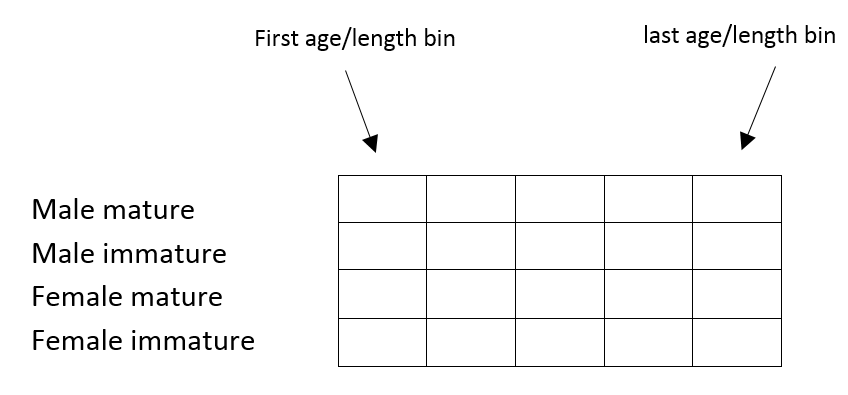
\includegraphics[scale=0.3]{Figures/partition.png}
		\caption{A visual representation of a partition}\label{Fig:part}
\end{figure}

So they define four time steps, labelled 1 through 4. Step 1 includes the non-spawning fishery. Step 2 includes the migration to the spawning area. Step 3 includes the spawning fishery. Step 4 includes recruitment and the migration back to the non-spawning area. (In fact, they could have used only 3 time steps, by using a single step in place of their steps 2 and 3. Because the default order of processes within a time step places migrations before fisheries, the processes would still have occurred in the right order.) There are other details to be sorted out, such as the proportion of natural mortality occurring in each time step and where observations occur, but this gives the basic idea.

This structure can be used to implement complex models, with intermingling of separate species and stocks, with complex migration patterns over multiple areas, and multiple sources of anthropogenic impact using different methods and covering different areas and times. However, we note that there is little point in using a complex structure to model a population when there are no observations to support that structure. In other words, use a structure for your model that is compatible with the data available. For information on how to define categories and using \CNAME's shorthand syntax see Section~\ref{sec:ShorthandSyntax-section}.

The model is run from an initial year up to the final(current) year. It can also be run past the final year to make projections --- things that happen in the future --- up to the final projection year.

An example, to specify a model with 2 categories (male and female) with ages 1-20 (with the last age a plus group) and an age-length relationship defined with the label \texttt{male\_growth} and \texttt{female\_growth}, then the \texttt{@model} example from above becomes,
{\small{\begin{verbatim}
		@model
		start_year
		final_year
		min_age 1
		max_age 20
		age_plus_group True
		initialisation_phases iphase
		time_steps step1 step2
\end{verbatim}}}

\subsection{\I{The state object and the partition}}

The key component of the state object is the partition, a matrix that store numbers of individuals at age for each category. A category represents a group of individuals that have the same specific attributes, examples of such attributes include life histories and growth rates, etc. For example, categories may include labels such as:

\begin{itemize}
\item Sex (male or female);
\item Area (any number of areas, named by the user);
\item Maturity (immature or mature);
\item Growth-path (any number of growth-paths);
\item Tag (any number of tagging events);
\item Species
\end{itemize}

A stock can be thought of as a population of individuals which recruits separately. See Section \ref{sec:maturity-notinpartition} for the treatment of maturity when it is not a category in the partition. 

So, you need to tell \CNAME\ the following: 

\begin{itemize}
\item	The minimum and maximum age classes in an age-based model.
\item	Whether there is an age-plus group.
\item The names of all categories.
\end{itemize}

Age classes are always one year wide, except that the maximum age group can optionally be a plus group. Users need to choose the minimum and maximum age classes. 

\CNAME\ allows categories of the partition to exist for certain years of the model. This is added for computational efficiency, when models contain a large number of categories that do not persist for all model years. Situations where this is beneficial is when a model contains a process that does a one off transition of fish from one category into another category in a subset of the model initialisation phases or years (for example, tagging events). Excluding categories for certain years can save a considerable amount of time as CASAL2 does not need to, for example, initialising empty categories or implement processes in time periods when they have no effect. 

Another important component of the state object in \CNAME\ are derived quantities. This includes quantities such as a mature biomass (for example, in fisheries models, the mid-spawning season biomasses of spawning fish, SSB) for either one or sum of more than one category. \CNAME\ derives through the command \command{derived\_quantity}, and may be required in the specification of some processes (i.e., in fisheries models, a recruitment process that  specifies a stock recruitment relationship requires the definition of a derived quantity that specifies the mid-season spawning stock biomass).

\subsection{\I{Time sequences}}

The time sequence of the model is defined in the following parts;
\begin{itemize}
  \item \I{Annual cycle}
  \item \I{Initialisation}
  \item \I{Model run years}
  \item \I{Projection year}s
\end{itemize}

\subsubsection*{\I{Annual cycle}}

The annual cycle is implemented as a set of processes that occur, in a user-defined order, within each year. Time-steps are used to break the annual cycle into separate components, and allow observations to be associated with different time periods and processes. Any number of processes can occur within each time-step, in any order (although there are limitations around mortality based processes - see Section~\ref{sec:mortality_block}) and can occur multiple times within each time-step. Note that time-steps are not implemented during the initialisation phases (effectively, there is only one time-step), and that the annual cycle in the initialisation phases can, optionally, be different from that which is applied during the model years.

\subsubsection*{\I{Mortality blocks}}\label{sec:mortality_block}

For every time step in an annual cycle there is an associated \emph{mortality block}. Mortality blocks are a key concept in \CNAME.

Mortality blocks are used to define the `point' in the model time sequence when observations (see Section~\ref{sec:observation-section}) are evaluated, and derived quantities (see Section~\ref{sec:derived-quantities}) are calculated.

A mortality block is defined as a consecutive sequence of mortality processes within a time step. The processes that are mortality processes are all pre-defined in \CNAME, and cannot be modified. These include all the processes described in subsection~\ref{sec:mortality}. 

\CNAME\ requires that each time step has exactly one mortality block. The achieve this, either all the mortality processes in a time step must be sequential (i.e., there can not be a non-mortality process between any two mortality processes within any one time step); or if no mortality processes occur in a time step then the mortality block is defined to occur at the end of the time step. 

\CNAME\ will error out if more than one mortality block occurs in a single time step. 

\begin{figure}[H]
	\centering
	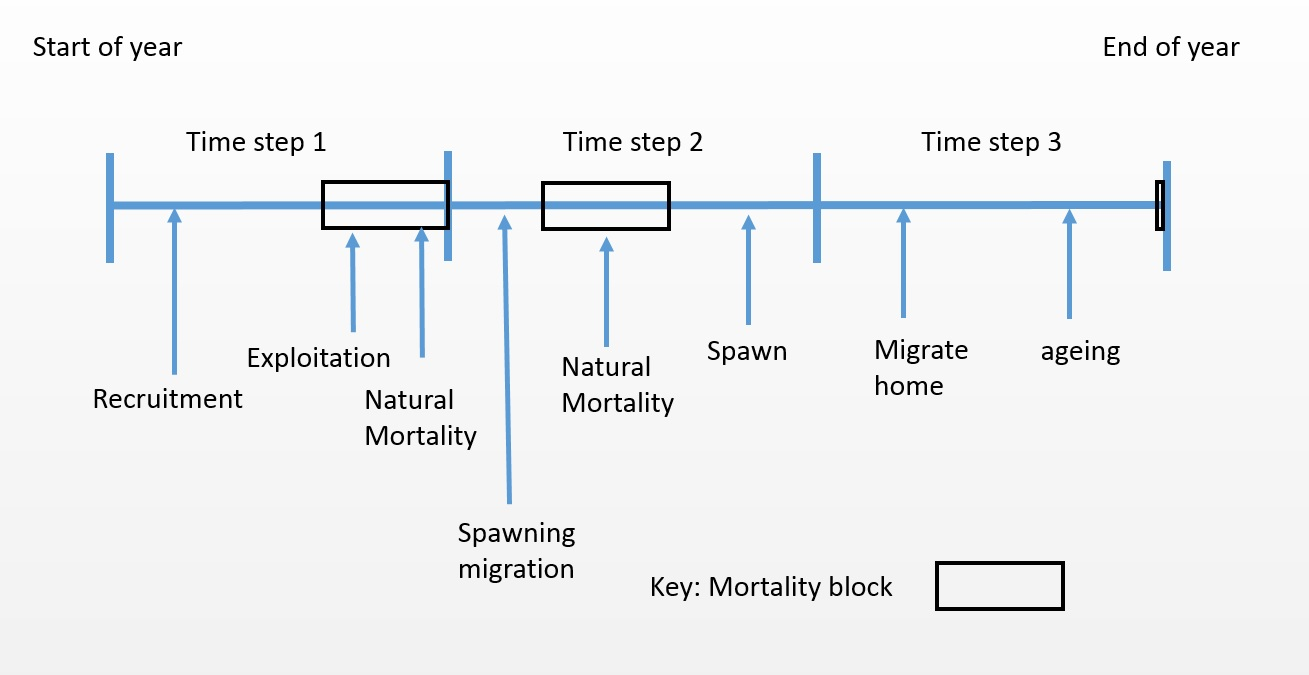
\includegraphics[scale=0.5]{Figures/annual_cycle.jpg}
	\caption{A visual representation of a hypothetical sequence for an annual cycle.}\label{Fig:annual}
\end{figure}

\subsubsection{\I{Initialisation}}

Initialisation is the process of determining the model equilibrium starting state, or some other initial state for the model, prior to the start year of the model.

There are multiple methods to initialise a partition in \CNAME. These methods are: iterative, fixed, derived, and Cinitial. 

Model initialisation can also occur in several phases\index{Initialisation!phases}, each of which can be a different method. These are carried out in sequence. At the end of all of the initialisations, \CNAME\ then runs the model years carrying out processes in each time step in the annual cycle.

The multi-phased initialisation allows the user to choose a number of initialisations that may assist with optimising the models for speed, initialise a non-equilibrium starting state, or resolve simple processes before introducing more complex ones.

Each phase of the initialisation defaults to have the same processes and in the same order as defined in the annual cycle. Although they can involve any number of processes using the \texttt{insert\_processes} subcommand.

In each initialisation phase, the processes defined for that phase are carried out and used as the starting point for the following phase or, if it is the last phase, then the years that the model is run over. 

Note that the \emph{first} initialisation phase is always initialised with each element (i.e., each age and category) set at zero. Note that you may need to be careful when using complex category inter-relationships or density dependent processes that depend on a previously calculated state, as they may fail when used in the first phase of an initialisation. 

Multi-phase iterations\index{Multi-phase iteration} can also be used to determine if the initialisation has converged. Here, add a second initialisation phase for, say, $1$ year (with the same processes applied). Then report the state at the end of the first and second phase. If these states are identical, then its likely that the initialisation has converged to an equilibrium state.

Syntax for including or excluding processes through the \texttt{insert\_processes} and  \texttt{exclude\_processes}. For the \texttt{insert\_processes} the syntax is;
{\small{\begin{verbatim}
		insert_processes time_step_label(process_label_in_annual_cycle) = label_new_process
\end{verbatim}}}
		An example of this is would be in the \command{time\_step} labelled \texttt{Oct\_Nov} include the \command{process} labelled \texttt{predationIni} before the \command{process} labelled \texttt{Instantaneous\_Mortality}
{\small{\begin{verbatim}
		insert_processes Oct_Nov(Instantaneous_Mortality)=predationIni
\end{verbatim}}}

if you want to include a process at the end of the time step you can use the following syntax,
{\small{\begin{verbatim}
		insert_processes Oct_Nov()=predationIni
		\end{verbatim}}}
To exclude a process from an initialisation phase the syntax is much simpler and can be done by the following subcommand in your \command{initialisation\_phase};

{\small{\begin{verbatim}
		exclude_processes process_label_in_annual_cycle
    	exclude_processes Instantaneous_Mortality	
		\end{verbatim}}}

The command above will remove the process \texttt{Instantaneous\_Mortality} during that particular initialisation phase.

\subsubsection*{\I{Iterative Initialisation}}

The iterative initialisation is a general solution for initialising the model. The iterative method can be slow to converge, depending on the nature of the problem being resolved, but will work on even complex structured models that may be difficult or impossible to implement using analytic approximations. 

The number of iterations in the iterative initialisation can effect the model output, and these should be chosen to be large enough to allow the population state to fully converge. We recommend that a period of about two generations to ensure convergence. \CNAME\ can be requested to report a number of convergence statistics that can assist the user determine the level of convergence.

In addition, the iterative initialisation phase can optionally be stopped early if some user defined convergence criteria is met. For list of supplied years in the initialisation phase, convergence is defined as met if the proportional absolute summed difference between the state in year $t-1$ and the state in year $t$ ($\widehat{\lambda}$) is less than a user defined $\lambda$ where, 
\begin{equation}
  \widehat{\lambda} = \frac{\sum\limits_{i} \sum\limits_{j} \left|\text{element}(i,j)_t - \text{element}(i,j)_{t-1} \right|}{\sum\limits_{i} \sum\limits_{j} \frac{}{}\text{element}(i,j)_t}
\end{equation}

Hence, for an iterative initialisation you need to define;
\begin{itemize}
  \item The initialisation phases.
  \item The number of years in each phase and the processes to apply in each (default is the annual cycle).
\end{itemize}

\subsubsection*{\I{Derived Initialisation}}

\texttt{Derived} initialisation is an analytical solution that calculates the equilibrium age structure and the plus group using a geometric series solution. The benefit of this method is it can be solved in max\_age - min\_age +1 years, so is computationally faster than the iterative initialisation phase. Users should be warned that we have found under some process combinations (for example. one way migrations) that this solution does not reach the exact equilibrium partition. We note that if using this method, that users confirm the partition has reached an equilibrium state by either comparing with and iterative initialisation, or by adding a second iterative initialisation phase of a limited number of iterations to confirm convergence.

\subsubsection*{\I{Cinitial Initialisation}}

This initialisation is only available as a second or greater phase initialisation, and can only be applied after derived or iterative initialisation phases. The Cinitial factors that can be estimated to shift the initial population away from an equilibrium state prior to start year. If there is known exploitation before data exists for a population this can be a solution for estimating a non equilibrium population. Note that it may be advisable to include an observation of age composition data for the first year of the model in order to estimate the non equilibrium population state. 

\subsubsection*{\I{Fixed Initialisation}}

This is a user defined table that is taken to be the initial partition prior to the start year. Users have the ability to initialise models by specify the numbers at age for each category. Be careful when initialising models with this type, if the model applies processes that require derived quantities to be calculated in the initialisation phase. As this may cause undefined behaviour.

\subsection{\I{Model run years}}

Following initialisation, the model then runs over a number of user-defined years from (initial\_year to final\_year). For this part of the model, the annual cycle can be broken into separate time-steps, and observations can be associated with the state of the model at the end of any time-step, i.e., likelihoods for particular observations are evaluated, if required, within each time-step. 

Processes are carried out in the order specified within each time-step. These can be the same or different to the processes in initialisation phases of the model. 

The run years define the years over which the model is to run and the annual cycle within each year. The model runs from the start of year \argument{initial} and runs to the end of year \argument{current}. The projection part then extends the run time up to the end of year \argument{final}. 
\begin{itemize}
  \item The time-steps and the processes applied in each
  \item The initial year (i.e., the model start year)
  \item The final year (i.e., the model end year)
  \item The projection final year (i.e., the model projection end year)
\end{itemize}

\subsection{\I{Projection years}}\label{sec:projection}

Projecting is the process of running the model forwards into the future, using stochastic and or deterministic values for population dynamic parameters, such as recruitments and catches. Users invoke \CNAME\ to run in projection mode using the following command \texttt{casal2 -f 1}. The number the follows the \texttt{-f} parameter indicates how many projections you would like to undertake for each set of parameters supplied. This allows you to explore many future scenarios for a single set of parameters, this should only be used if you are applying a projection type that is stochastic.

Projection years occur immediately after the model run years.

In a projection run in \CNAME\, a model is initialised and run through the model years from \argument{initial} to the \argument{final}. Then, the model is re-run from \argument{initial} to \argument{projection\_final\_year}, where any parameter can be either fixed or, if specified, drawn from a stochastic distribution or process during that time period. This gives users the ability to apply projection methods on parameters that occur between \argument{start\_year} and \argument{final\_year} defined in teh \command{model} block. An example of when users may want to do this is when you are estimating all the year class parameters. Usually the last few year class parameters are poorly estimated, although this depends on the quality and coverage of the compositional data that would inform these parameter. So users may wish to assume they are unknown and apply projection methods as they do for future values.

\CNAME\ does not have any default projections for when parameters are specified by year. These must be specified using the \command{project} command blocks. This is important for parameters that may vary from year to year (such as year class strength parameters), \CNAME\ should error out if users do this.

\CNAME\ allows any estimable parameter to be specified in a \command{project} block and then used in a projection. The available projection types for these parameters include constant, lognormal, empirical-lognormal, or empirical re-sampling.

The subcommand that is common to all projection methods is the \argument{multiplier} command. This is as it suggests a constant that is multiplied to the projected value after it has been derived by its respective method.

A \textbf{note} to users for the specific year class parameter, The definition of year applies to the \argument{ycs\_years} not the model years. As defined in Section~\ref{subsubsec:BH-recruitment}, \argument{ycs\_years} are offset between time of spawning and when they enter the partition. 

\paragraph*{Constant}
A parameter can either be fixed during all projection years or specified individually for each projection year. This is a deterministic assumption, where the parameter is assumed to be known without error during projection years.

{\small{\begin{verbatim}
		@project Future_ycs
		type constant
		parameter process[Recruitment].ycs_values
		years 2012:2016
		values 1 2 1 2 0.5
		multiplier 1
		\end{verbatim}}}
\paragraph*{Empirical resampling}

Parameters that have time components associated with them can be re-sampled uniformly with replacement over a range of years and used as the projected year values. The year range which users must specify are between \argument{start\_year} and \argument{final\_year}
{\small{\begin{verbatim}
		@project Future_ycs
		type empirical_sampling
		parameter process[Recruitment].ycs_values
		years 2012:2016
		start_year 1988
		final_year 2008
		multiplier 1
		\end{verbatim}}}


\paragraph*{Lognormal}
The parameters are originally drawn from a gaussian distribution in log space and exponentiated out to form the lognormal distribution,
\begin{equation}\label{eq:lognormal}
X_p = e^{\epsilon_p- 0.5\sigma^2}
\end{equation}
where $\epsilon_p\stackrel{iid}{\sim}N(\mu,\sigma)$ and $X_p$ is the projected value for parameter $X$, and $\mu$, $\sigma$ is the mean and standard deviation on the log scale. An example of applying this process is if we wanted to draw future year class parameters from a lognormal distribution with mean 1 and standard deviation 0.8, we would define the syntax as,
 
 {\small{\begin{verbatim}
 		@project Future_ycs
 		type lognormal
 		parameter process[Recruitment].ycs_values
 		years 2012:2016
 		mean 0
 		sigma 0.8
 		multiplier 1
 		\end{verbatim}}}


\paragraph*{Lognormal-Empirical}
This class applies Lognormal draw as in the \argument{LogNormal} class but it allows the user to specify a year range which is re-sampled uniformly without replacement. These re sampled values are then used to calculate the standard deviation of the distribution. Then equation~\eqref{eq:lognormal} is used to generate future values with user defined $\mu$ and empirically calculated $\sigma$,

{\small{\begin{verbatim}
		@project Future_ycs
		type lognormal_empirical
		parameter process[Recruitment].ycs_values
		years 2012:2016
		mean 0
		start_year 1988
		final_year 2008
		multiplier 1
		\end{verbatim}}}


\subsection{\I{Population processes}}

Population processes are those processes that change the model state. Processes produce changes in the model partition, by adding, removing or moving individuals between ages and/or categories. The population processes include recruitment\index{Recruitment}, ageing\index{Ageing},  mortality\index{Mortality} events (e.g., natural and anthropogenic) and category transition processes\index{Category transition} (i.e., processes that move individuals between categories while preserving their age structure). See Section~\ref{sec:population-section} for a complete list of available processes.

There are two types of processes, processes that occur across multiple time steps in the annual cycle e.g Natural Mortality and Instantaneous Mortality. There are also processes that only occur within the time step they are defined. Each of these processes is carried out in the user-defined prescribed order when initialising the model, and then for a user-defined order in each year in the annual cycle\index{Annual cycle}. 

\subsubsection{\I{Recruitment}}

Recruitment processes are defined as a process that introduces new individuals into the partition. \CNAME\ currently implements two types of recruitment process, constant recruitment\index{Recruitment ! Constant} and  \I{Beverton-Holt recruitment}\index{Recruitment ! Beverton-Holt} \citep{1203}.

In the recruitment processes, the number of individuals are added to a single age class within the partition, with the amount defined by the type of recruitment process and its function. If more than one category is defined, then the proportion of recruiting individuals to be added to each category is specified by the \argument{proportions} parameter, or multiple recruitment processes can be defined. For example, if recruiting to categories labelled male and female, then you might set the proportions as $0.5$ and $0.5$ respectively to denote that half of the recruits recruit to the male category and the remaining half to the female category. 

\hl{An important note here is that recruitment can differ from a spawning event or the creation of a cohort/year class. In a fisheries context recruitment usually refers to indivisuals 'recruiting' to the fishery. This is done for a few reasons, one being often we do not have a lot of information relating to age classes between spawning and data collection i.e. an information gap exists. Once again in a fisheries context this information gap can refer to the time between spawning and being vulnerable to a survey or fishery for data collection. Thus users may only want to model the population for which data is available. This offset between spawning and recruitment is parameratised either by the recruitment variable \texttt{age} or \texttt{min\_age} (the default value for the \texttt{age} parameter in the recruitment process). For CASAL users the parameter \texttt{age} is the same as \texttt{y\_enter} in CASAL.}. 

For the constant and Beverton-Holt recruitment processes, the  number of individuals following recruitment in year $y$ is,  

\begin{equation}
N_{y,a,j} \leftarrow N_{y,a - 1,j} + p_j(R_{y,a})
\end{equation}
where $N_{y,a,j}$ is the numbers in category $j$ at age $a$, $p_j$ is the proportion to category $j$, and $R_{y,a}$ is the number of recruits for year $y$. See below for how $N_{y,a,j}$ is determined in each of these cases.

\subsubsection*{\I{Constant Recruitment}}

In the constant recruitment process the total number of recruits added each year $y$ in age $a$ is $R_{y,a}$, and is simply $p_j(R_0)$, i.e.
\begin{equation}
  R_{y,a,j} = p_j(R_0)
\end{equation}

Constant recruitment recruits a constant number of individuals each year. It is equivalent to a Beverton-Holt recruitment process with steepness set equal to one (i.e., $h=1$).

For example, to specify a constant recruitment process, where individuals are added to male and female immature categories at $age=1$ evenly (\texttt{proportions} = 0.5), and the number to add is $R_0=5 \times 10^5$, then the syntax is

{\small{\begin{verbatim}
	@process Recruitment
	type constant_recruitment
	categories male.immature female.immature
	proportions 0.5 0.5
	r0 500000
	age 1
\end{verbatim}}}

\subsubsection*{\I{Beverton-Holt recruitment}}\label{subsubsec:BH-recruitment}

In the Beverton-Holt recruitment process the total number of recruits added each year is $R_y$, and is the product of the average recruitment $R_0$, the annual year class strength multiplier, $YCS$, and the stock-recruit relationship i.e.,
\begin{equation}\label{eq:BH}
  R_{y,a,j} = p_j(R_0 \times YCS_{ycs\_year} \times SR(SSB_{ycs\_year}))
\end{equation}
where
\begin{equation}\label{eq:year_class}
ycs\_year = y - \texttt{ssb\_offset}
\end{equation}

where $a$ is the parameter \texttt{age}, $p_j$ is the proportion of recruits to enter category $j$ and \texttt{ssb\_offset} is the lag between spawning and recruitment. As stated earlier recruitment refers to the recruitment into the population and may differ from the spawning event. See two paragraphs below on more information about \texttt{ssb\_offset}, but in general this parameter shouldn't be specified by the user.

$SR$ is the Beverton-Holt stock-recruit relationship parametrised by the steepness $h$,
\begin{equation}\label{eq:BH_SR}
SR(SSB_y) = \frac{SSB_y}{B_0} / \left( 1-\frac{5h-1}{4h} \left( 1-\frac{SSB_y}{B_0} \right) \right)
\end{equation}

Note that the Beverton-Holt recruitment process requires a value for \Bzero\ and $SSB_y$ to resolve the stock-recruitment relationship. Here, a derived quantity (see Section \ref{sec:derived-quantities}) must be defined that provides the annual $SSB_y$ for the recruitment process. \Bzero\ is then defined as the value of the $SSB$ at the end of one of the initialisation phases, this initialisation phase is defined by the parameter \texttt{b0\_intialisation\_phase}. During initialisation the $YCS$ multipliers are assumed to be equal to one, and recruitment that happens in the initialisation phases that occur before and during the phase when \Bzero\ is determined is assumed to have steepness $h=1$ (i.e. in those initialisation phases, recruitment is simply equal to \Rzero). Recruitment in the initialisation phases after the phase where \Bzero\ was determined follow the Beverton-Holt stock-recruit relationship defined above. \Rzero\ and \Bzero\ have a direct relationship when there are no density dependent processes in the annual cycle, for this reason users can choose to initialise models using \Bzero\ or \Rzero.

\texttt{ssb\_offset} should not be manually given by the user in commonplace, \CNAME\ determines \texttt{ssb\_offset} by the order of ageing, recruitment, spawning and the recruitment parameter \texttt{age}, 
\begin{itemize}
	\item If recruitment then ageing then spawning, then \texttt{ssb\_offset} should equal \texttt{age} + 1.
	\item If spawning then ageing then recruitment, then \texttt{ssb\_offset} should equal \texttt{age} - 1.
	\item else \texttt{ssb\_offset} = \texttt{age}
\end{itemize}

The certain scenarios where the user will manually want to input these values is if there are multiple ageing processes in the annual cycle. We have not coded \CNAME\ to deal with this situation so will be up to the user to define the \texttt{ssb\_offset}.

Another important input parameter is the \texttt{ycs\_years} which is defined in Equation~\eqref{eq:year_class}. When referencing the parameter \texttt{ycs\_values} you should always reference it by the \texttt{ycs\_years} parameter, this is important to note for when defining \command{estimate}, \command{project} and \command{time\_varying} blocks for the parameter \texttt{ycs\_values}. An example follows

Year classes values are standardised using the Haist parametrisation suggested by V. Haist. Here, the model parameter \texttt{ycs\_values} is a vector \textbf{Y}, covering years from \texttt{start\_year} - \texttt{ssb\_offset} to \texttt{final\_year} - \texttt{ssb\_offset}, as defined by the parameter \texttt{ycs\_years}. The year class strengths are calculated by $YCS_i=Y_i/\bar{\textbf{Y}}$ where the mean is calculated over the user-specified years \texttt{standardise\_ycs\_years}. Then,
\[
YCS_i = 
\begin{cases}
Y_i / mean_{y \in S}(Y_y) & :y \in S\\
Y_i					 & :y \notin S
\end{cases}
\]

where S is the set of years from \texttt{standardise\_ycs\_years}. One effect of this parametrisation is that\Rzero\ is then defined as the mean estimated recruitment over the years S, because the mean year class multiplier over these years will always be one.

Typically, the user will define \texttt{standardise\_ycs\_years} to span the years for which they expect to have reasonable estimates of YCSs. Often, the user will wish to force $Y_y=1$ for some or all years $y\in S$ (this is equivalent to forcing Ry=R0 x SR) by setting the lower and upper bounds of these Ys to be 1. An exception to this might occur for the most recent YCSs, which the user may want to estimate, but not include in the definition of R0 (because the estimates are based on too few data). Note that, optionally, the user may exclude one or more years from within the range from the averaging process of the Haist parameterisation. 

The advantage of the Haist parameterisation is that the user need no longer use a large penalty to force the mean of the YCS parameter to be 1 (though they should still use a small penalty to stop the mean of Y from drifting). This may improve MCMC performance.  projected YCS are not affected by this feature. A disadvantage with this parameterisation in a Bayesian analysis is that the prior refers to the Y’s, not the YCS.

An example of a the configuration of the Beverton-Holt recruitment process, where individuals are added to the category `immature' at $age=1$, and the number to add is $R_0=5 \times 10^5$. \texttt{SSB\_derived\_quantity} is a derived quantity that specifies the total spawning stock biomass that contributed to the this year class, with \Bzero\ the value of the derived quantity at the end of the initialisation phase labelled \texttt{phase1}. The $YCS$ are standardised to have mean one in the period 1995 to 2004, and recruits enter into the model two years following spawning.


{\small{\begin{verbatim}
	@process Recruitment
	type recruitment_beverton_holt
	categories immature
	proportions 1.0
	r0 500000
	b0_initialisation_phase phase1
	steepness 0.75
	age 1
	ssb SSB_derived_quantity
	standardise_ycs_years 1995:2004
	ycs_years 1994 1995 1996 1997 1998 1999 2000 2001 2002 2003 2004 2005 2006
	ycs_values   0.65    0.87    1.6    1.13    1.0235    0.385   2.653    1.35    1    1    1    1    1
\end{verbatim}}}

So, to specify a Beverton-Holt recruitment for each stock, the following information is required:
\begin{enumerate}
	\item YCS, starting from year (\texttt{start\_year} - \texttt{ssb\_offset}) and extending up to year (\texttt{final\_year} - \texttt{ssb\_offset}).
	\item The value of \texttt{age} aka \texttt{y\_enter} to CASAL users.
	\item the steepness parameter \texttt{h}.
	\item In a multi category model, the proportion of recruits for each category.
	\item label for the derived quantity
\end{enumerate}
\subsubsection{\I{Ageing}\label{sec:ageing}}

The ageing process `ages' individuals --- it simply moves all individuals in the named categories $i$ to the next age class $j + 1$, or accumulates them if the last age class is a plus group. 

The ageing process is defined as,
\begin{equation}
  \text{element}(i,j) \leftarrow \text{element}(i,j-1)
\end{equation}

except that in the case of the plus group (if defined), 
\begin{equation}
  \text{element}(i,age_{\text{max}}) \leftarrow \text{element}(i,age_{\text{max}}) + \text{element}(i,age_{\text{max}-1}).
\end{equation}

For example, to apply ageing to the categories \texttt{immature} and \texttt{mature}, then the syntax is,

{\small{\begin{verbatim}
	@process Ageing
	type ageing
	categories immature mature
	\end{verbatim}}}

Note that ageing is \emph{not} applied by \CNAME\ by default. As with other processes, \CNAME\ will not apply a process unless its defined and specified as a process within the annual cycle. Hence, it is possible to specify a model where a category is not aged. \CNAME\ will not check or otherwise warn if there is a category defined where ageing is not applied.

\subsubsection{\I{Mortality}\label{sec:mortality}}

Six types of mortality processes are permissible in \CNAME, constant rate, event, biomass-event, Hollings mortality, initialisation mortality event and instantaneous. These processes remove individuals from the partition, either as a rate, as a total number (abundance), as a biomass of individuals or as a mixture of these. Note that \CNAME\ does not (yet) implement the Baranov catch equation. To apply both natural and biomass-event mortality, users can use \texttt{mortality\_instantaneous}. Note that all mortality processes occur within a mortality block of a time step see Section~\ref{sec:mortality_block} for more information and definitions on mortality blocks. 

\paragraph{Constant mortality rate}

To specify a constant annual mortality rate \index{Constant mortality}($M=0.2$) for categories `male' and `female', then, 
{\small{\begin{verbatim}
@process NaturalMortality
type mortality_constant_rate
categories male female
selectivities One One
m 0.2 0.2
\end{verbatim}}}

\begin{equation}
D_{j,t} = \sum_a N_{a,j} (1 - \exp{S_{a,j} M_j p_t})
\end{equation}
Where, $D_{j,t}$ is the number of deaths in category $j$ in time step $t$, $N_{a,j}$ is the number of individuals in category $j$ at age $a$. $S_{a,j}$ is the selectivity value for age $a$ in category $j$, $M_j$ is the mortality rate for category $j$, and $p_t$ is the proportion of the mortality rate to apply in time step $t$.

Note that the mortality rate process requires a selectivity. To apply the same mortality rate over all age classes, use a selectivity defined as $S_j=1.0$ for all ages $j$, e.g.,

{\small{\begin{verbatim}
@selectivity One
type constant
c 1
\end{verbatim}}}

\paragraph{Event and biomass-event mortality}

The event mortality process\index{Event mortality} and biomass mortality\index{Biomass event mortality} processes act in a similar manner, except that they remove a specified abundance (number of individuals) or biomass respectively. These can be used to include anthropogenic mortality where numbers of removals are known, for example, fishing in a fisheries model, rather than applying mortality as a rate. 

In these cases, the abundance or biomass removed is also constrained by a maximum exploitation rate. \CNAME\ removes as many individuals or as much biomass as it can while not exceeding the maximum exploitation rate. When minimising, event mortality processes require a penalty to discourage parameter values that do not allow the defined number of individuals to be removed. Here, the model penalises those parameter estimates that result in an too low a number of individuals in the defined categories (after applying selectivities) to allow for removals at the maximum exploitation rate. See Section \ref{sec:penalties} for more information on how to specify penalties.

For example, the event mortality applied to user-defined categories $i$, with the numbers removed at age $j$ determined by a selectivity-at-age $S_j$ is applied as follows:

First, calculate the vulnerable abundance for each category $i$ in $1 \ldots I$ for ages $j = 1 \ldots J$ that are subject to event mortality,
\begin{equation}
  V(i,j) = S(j) N(i,j)
\end{equation}

And hence define the total vulnerable abundance $V_{total}$ as,
\begin{equation}
  V_{total}  = \sum\limits_i {\sum\limits_j {V(i,j)}} 
\end{equation}

Hence the exploitation rate\index{Maximum exploitation rate} to apply is 
\begin{equation}
U = \begin{cases}
  C/V_{total}, & \text{if $C/V_{total} \leq U_{max}$} \\
  U_{max}, & \text{otherwise}\\ 
  \end{cases} 
\end{equation}

And the number removed $R$ from each age $j$ in category $i$ is,
\begin{equation}
  R(i,j) = UV(i,j)
\end{equation}

For example, to specify fishing mortality in a fisheries model, with catches given for a set of specific years, over categories `immature' and 'mature', with selectivity `FishingSel' and assuming a maximum possible exploitation rate of 0.7, then the syntax would be,

{\small{\begin{verbatim}
	@process Fishing
	type event_mortality
	categories immature mature
	years 2000 2001 2002 2003
	U_max 0.70
	selectivities FishingSel FishingSel
	penalty event_mortality_penalty
	\end{verbatim}}}

\paragraph{Instantaneous mortality}

The instantaneous mortality process\index{Instantaneous mortality} is a process that combines both natural mortality and event biomass mortality into a single process. This allows the natural mortality to occur occurs across multiple time steps, and can specify multiple instances of event mortality to account for, say, multiple fisheries operating sequentially or concurrently. This process applies half the natural mortality in each time step, then the mortalities from all the concurrent fisheries instantaneously, then the remaining half of the natural mortality.

When instantaneous mortality is applied the following equations are used.

\begin{itemize}
	\item An exploitation rate (actually a proportion) is calculated for each fishery, as the catch over the selected-and-retained biomass,
	$$ U_f = \frac{C_f}{\sum_j \bar{w}_jS_{f,j}n_j e^{-0.5tM_j}}$$
	\item The fishing pressure associated with fishery $f$ is defined as the maximum proportion of fish taken from any element of the partition in the area affected by fishery $f$,
	$$ U_{f,obs} = max_j(\sum_k S_{k,j}U_k) $$
	where the maximum is over all partition elements affected by fishery $f$, and the summation is over all fisheries $k$ which affect the jth partition element in the same time step as fishery $f$.
	
In most cases the fishing pressure will be equal to the exploitation rate (i.e., $U_{f,obs} = U_f$), but they can be different if (a) there is another fishery operating in the same time step as fishery $f$ and affecting some of the same partition elements, and/or (b) the selectivity $S_{f,j}$ does not have a maximum value of 1.
	
There is a maximum fishing pressure limit of $U_{f,max}$ for each fishery $f$. So, no more than proportion $U_{f,max}$ can be taken from any element of the partition affected by fishery $f$ in that time step. Clearly $0 \leq U_{max} \leq 1$. It is an error if two fisheries which affect the same partition elements in the same time step do not have the same $U_max$.

For each $f$, if $U_{f,obs} > U_{f,max}$, then $U_f$ is multiplied by $U_{f,max}/U_{f,obs}$ and the fishing pressures are recalculated. In this case the catch actually taken from the population in the model will differ from the specified catch, $C_f$.
	
\item The partition is updated using
	$$ n'_j = n_j exp(-tM_j)\big[1 - \sum_f S_{f,j} U_f \big] $$ 
\end{itemize}

An example of the syntax is if we want to apply natural mortality of $0.20$ across three time steps on both male and female categories. And we have two method of removals (fisheries) \texttt{FishingWest FishingEast} with there respective catches known for years 1975:1977 in kilograms. These are given in the \texttt{catches} table and information on selectivities, penalties and maximum exploitation rates are given in the \texttt{fisheries} table.

{\small{\begin{verbatim}
	@process instant_mort
	type mortality_instantaneous
	m 0.20
	time_step_ratio 0.42 0.25 0.33
	selectivities One
	categories male female
	units kgs

	table catches
	year FishingWest FishingEast
	1975	80000	111000
	1976	152000	336000
	1977	74000	1214000
	end table

	table method
	method       category  selectivity u_max   time_step penalty
	FishingWest   stock     westFSel    0.7     step1     CatchPenalty
	FishingEast   stock     eastFSel    0.7     step1     CatchPenalty
	end_table
	\end{verbatim}}}

\paragraph{Hollings mortality rate}

The density-dependent Holling mortality process\index{Holling mortality} applies the Holling Type II and Type III functions \citep{Holling1959}, but is generalised using the Michaelis-Menten equation \citep{MentenMichaelis1913}. The function removes a number or biomass from a set of categories according to their total (selected) abundance (or biomass)and some 'predator' abundance (or biomass), but constrained by a maximum exploitation rate.

For example, the mortality applied to user-defined categories $k$, with the numbers removed at age $l$ determined by a selectivity-at-age $S(l)$ is applied as follows:

First, calculate the total predator abundance (or biomass) over all predator categories $k$ in $1 \ldots K$ and ages $l = 1 \ldots L$ that are applying the mortality,
\begin{equation}
	P(k,l) = S_{predator}(l) N_{predator}(k,l)
\end{equation}

And define the total predator abundance (or biomass) $P_{total}$ as,
\begin{equation}
	P_{total}  = \sum\limits_K {\sum\limits_L {P(k,l)}} 
\end{equation}

Then, calculate the total vulnerable abundance (or biomass) over all prey categories $k$ in $1 \ldots K$ and ages $l = 1 \ldots L$ that are subject to the mortality,
\begin{equation}
	V(k,l) = S_{prey}(l) N_{prey}(k,l)
\end{equation}

And hence define the total vulnerable abundance (or biomass) $V_{total}$ as,
\begin{equation}
	V_{total}  = \sum\limits_K {\sum\limits_L {V(k,l)}} 
\end{equation}

and then, the the number to remove is determined as,
\begin{equation}
	R_{total} = P_{total} \frac{a  V_{total}^{x-1}}{b + V_{total}^{x-1}}
\end{equation}
where $x=2$ for Holling type II function,  $x=3$ for Holling type III function, or any value of $x \geq 1$ for the generalised Michaelis-Menten function, and $a > 0$ and $b > 0$ are the Holling function parameters.

Hence the exploitation rate\index{Maximum exploitation rate} to apply is 
\begin{equation}
	U = \begin{cases}
		R_{total}/V_{total}, & \text{if $R_{total}/V_{total} \leq U_{max}$} \\
		U_{max}, & \text{otherwise}\\ 
	\end{cases} 
\end{equation}

And the number removed $R$ from each age $l$ in category $k$ is,
\begin{equation}
	R(k,l) = UV(k,l)
\end{equation}

The density-dependent Holling mortality process is applied either as a biomass or an abundance depending on the value of the \texttt{is\_abundance} switch.

For example, a biomass Holling type II mortality process on \texttt{prey} by our predator \texttt{predator} would have syntax,

{\small{\begin{verbatim}
		@process HollingMortality
		type Holling_mortality_rate
		is_abundance F
		a 0.08
		b 10000
		x 2
		categories prey
		selectivities One
		predator_categories predator
		predator_selectivities One
		u_max 0.8
		\end{verbatim}}}

\paragraph{Initialisation event or biomass-event mortality}

The Initialisation event mortality process\index{Initialisation event mortality} are specific processes that only can occur in the initialisation phase. It allows users to apply abundance or biomass mortality events specifically in initialisation phases. This can be useful if you wanted to deviate a model from equilibrium before model start. This process applies a single catch for all iterations within the initialisation phase, this process wont apply any mortality outside of the initialisation phase. It is advised that users use this process in conjunction with the \texttt{insert\_processes} command in the \command{initialisation\_phase} block, and not embed this process in the annual cycle. Example syntax to implement such a scenario,

{\small{\begin{verbatim}
initialisation_phases Equilibrium_state Predation_state
time_steps Oct_Nov Dec_Mar

@initialisation_phase Equilibrium_state 
type derived

@initialisation_phase Predation_state
type iterative
insert_processes Oct_Nov()=predation_Initialisation

@process predation_Initialisation
type initialisation_mortality_event
categories male.HOKI female.HOKI
catch 90000
selectivities Hakesl Hakesl

time_step Oct_Nov
processes Mg1 Instantaneous_Mortality

@time_step Dec_Mar 
processes Recruitment Instantaneous_Mortality
\end{verbatim}}}

Note how we have added the \texttt{initialisation\_mortality\_event} into the initialisation phase \texttt{Predation\_state} but not in the annual cycle. This was a case where the functionality has been applied.



\subsubsection{\I{Transition By Category}}

This process covers moves individuals between categories. Because the \CNAME\ partition user defined, this type of process is used to move individuals between categorised, and is used to specify processes such as maturation (move individuals from an immature to mature state) or migration (move individuals from one area to another). 

\paragraph{Annual transition by category}

A special case is annual transition by category, which allows a transition to occur in a specific subset of years only, where each year can have a different rate.

In both cases, there has to be a one to one relationship between the `from' category and the `to' category --- for every source category there is one target category. If however, you want to merge categories, then just repeat the `to' category multiple times. 

\begin{equation}
	N_{a,j} = N_{a,i} \times P_i \times S_{a,i}
\end{equation}
where $N_{a,j}$ is the number of individuals that have moved to category $j$ from category $i$ in age $a$ and $N_{a,i}$ is the number of individuals in category $i$. $P_i$ is the proportion parameter for category $i$ and $S_{a,i}$ is the selectivity at age $a$ for category $i$.

An example, to specify a simple spawning migration of mature males from a western area migrating to an eastern (spawning) area, then the syntax is
{\small{\begin{verbatim}
		@process Spawning_migration
		type category_transition 
		from West.males	
		to East.males	
		selectivities MatureSel
		proportions 1
		\end{verbatim}}}

Where \texttt{MatureSel} is a selectivity that describes the proportion of age or length classes that are mature and thus move to the eastern area.

\subsubsection{\I{Tag Release events}}\label{sub:tag_release}

Tagging processes can be age or length based processes, where by numbers of fished are moved from an untagged category to a tagged category that the user has defined in the \command{Categories} block. Tag release processes can also account for tag induced mortality on individuals. Age based tag release events take a known number of individuals tagged for each age and do a straightforward category transition along with extra mortality. Length based tag release processes are more complicated, as \CNAME\ needs to calculate the age length matrix and exploitation by each length to then move the correct numbers at age based on the known lengths of release. \CNAME\ also allows for initial tag loss. An example of tag release by length process is as follows. 

{\small{\begin{verbatim}
		@process 2005Tags_shelf
		type tag_by_length 
		years 2005
		from male.untagged  female.untagged
		to male.2005  female.2005	
		selectivities MatureSel
		proportions 1
		selectivities ShelfselMale ShelfselFemale
		penalty tagging_penalty
		maximum_length 230
		plus_group False
		initial_mortality 0.1
		table proportions
		year 30 40 50 60 70 80 90 100 110 120 130 140 150 160 170 180 190 200 210 220
		2005  0 0 0.0580 0.1546 0.3380 0.1981 0.1643 0.0531 0.0242 0.0097 0 0 0 0 0 0 0 0 0 0
		end_table
		n 207
		U_max 0.999
		\end{verbatim}}}

The above process will move 207 individuals from a combination of male.untagged and female.untagged, based on the combination of growth rates and selectivity between the sexes.

\subsubsection{\I{Tag Loss}}

Tag Loss is the process where tags are lost from tagged categories over time from tag failure or getting knocked off. This process is applied as a instantaneous migration rate that can happen over multiple time steps in the annual cycle. This method assumes when tags are lost that the fish are transferred from the \subcommand{from} category to the \subcommand{to} category. How the tag loss rate is applied depends on whether the fish were only tagged with a single tag (\subcommand{tag\_number\_per\_animal = 1}), double tagged (\subcommand{tag\_number\_per\_animal = 2}) or $n$ tagged (\subcommand{tag\_number\_per\_animal = n}). The relationship is as follows

{\small{\begin{verbatim}
	@process Tag_loss
	type tag_loss
	categories tagged_fish
	tag_loss_rate 0.02
	time_step_ratio 0.25 0.75
	selectivities One
	tag_loss_type single
	year 1985
		\end{verbatim}}}

\subsection{\I{Derived quantities}\label{sec:derived-quantities}}

Some processes require, as arguments, a population value derived from the population state. These are termed \texttt{derived quantities}. Derived quantities are values, calculated by \CNAME\ at the end of a specified time-step in every year, and hence they have a single value for each year of the model. Derived quantities can be calculated as either an abundance or as a biomass. Abundance derived quantities are simply the count or sum of categories (after applying a selectivity). Biomass derived quantities are similar, except they are a measure of biomass. Derived quantities are also calculated during the initialisation phases, and hence the time-step during each phase must also be specified. If the initialisation time-steps are not specified, \CNAME\ will calculate the derived quantity during the initialisation phases in every year, at the end of the annual cycle. 

Derived quantities are required by some processes, for example the Beverton-Holt recruitment process. The Beverton-Holt recruitment process can require an equilibrium biomass ($B_0$) and annual spawning stock biomass values ($SSB_y$) to resolve the stock-recruit relationship. Here, these would be defined as the abundance or biomass of a part of the population at some point in the annual cycle for selected ages and categories, and would be calculated as a derived quantity.

Derived quantities are associated with a mortality block see section~\ref{sec:mortality_block} for more detail on mortality blocks. Users can ask for derived quantities partway through mortality blocks. Currently two methods are implemented in \CNAME\ to interpolate derived quantities part-way through a mortality block, these are \texttt{weighted\_sum} and \texttt{weighted\_product}, they are defined as,
\begin{itemize}
	\item \texttt{weighted\_sum}: after proportion $p$ of the mortality block, the partition elements are given by $n_{p,j} = (1 - p)n_j + p'_j$
	
	\item \texttt{weighted\_product}: after proportion $p$ of the mortality block, the partition elements are given by $n_{p,j} = n_j^{1-p} n'^p_j$
\end{itemize}
where, $n_p,j$ is the derived quantity at proportion $p$ of the mortality block for category $j$. $n_j$ is the quantity at the beginning of the mortality block and $n'_j$ is the quantity at the end of the mortality block.

As an example, to define a biomass derived quantity (say spawning stock biomass, SSB) for a model, evaluated at the end of the first time-step (labelled \texttt{step\_one}), over all 'mature' male and female categories and halfway through the mortality block using the \texttt{weighted\_sum} method, we would use the syntax,

{\small{\begin{verbatim}
@derived_quantity SSB
type biomass
time_step step_one
categories mature.male mature.female
selectivities One
time_step_proportion 0.5
time_step_proportion_method weighted_sum
\end{verbatim}}}

\subsection{\I{Age-length relationship}\label{sec:age-at-age}}

The age-length relationship defines the length at age (and the weight at length, see Section \ref{sec:mean-weight}) of individuals at age/category within the model. There are three length-age relationships available in \CNAME. The first is the naive no relationship (where each individual has length 1 irrespective of age). The second  and third are the von-Bertalanffy and Schnute relationships respectively. The length-at-age relationship is used to determine the length frequency, given age, and then with the length-weight relationship, a weight-at-age of individuals within an age/category. 

The three age-length relationships are,

\begin{description}
\item {None:} where the length of each individual is exactly 1 for all ages, in which case the \texttt{none} length-weight relationship must also be used.
\item{von Bertalanffy:}\index{von Bertalanffy growth curve} where length at age is defined as,
\begin{equation} 
\bar{s}(age)= L_\infty \left( 1 - \exp \left( -k \left(age-t_0 \right) \right) \right)
\end{equation}

\item{Schnute:}\index{Schnute growth curve} where length at age is defined as,
\begin{equation}
\bar{s}(age)=\displaystyle\begin{cases}
  \left[ y_1^b + (y_2^b - y_1^b) \dfrac{1-\exp \left(-a(age - \tau_1) \right)}{1-\exp \left(-a(\tau_2 - \tau_1) \right)} \right]^{1/b}, & \text{if $a\ne0$ and $b\ne0$} \\
  \AddVspace
  y_1 \exp \left[ \ln \left( y_2 / y_1 \right) \dfrac{1-\exp \left(-a(age - \tau_1) \right)}{1-\exp \left(-a(\tau_2 - \tau_1) \right)} \right], & \text{if $a\ne0$ and $b=0$} \\
  \AddVspace
  \left[ y_1^b + \left( y_2^b - y_1^b \right) \dfrac{age-\tau_1}{\tau_2 - \tau_1} \right]^{1/b}, & \text{if $a=0$ and $b\ne0$} \\
  \AddVspace
  y_1 \exp \left[ \ln \left( y_2/y_1 \right) \dfrac{age-\tau_1}{\tau_2 - \tau_1} \right] , & \text{if $a=0$ and $b=0$} \\
  \end{cases}
\end{equation}
\end{description}

The von Bertalanffy curve is parameterised by $L_\infty$, $k$, and $t_0$; the Schnute curve \citep{836} by $y_1$ and $y_2$, which are the mean lengths at reference ages $\tau_1$ and $\tau_2$, and $a$ and $b$ (when $b=1$, this reduces to the von Bertalanffy with $k=a$). 

When defining length-at-age in \CNAME, you must also define a length-weight relationship (see Section \ref{sec:mean-weight} below).

\subsubsection*{\I{Calculation of length-at-age (in an age-based model)}}

\subsubsection*{\I{Interpolation of length-at-age}}

\subsubsection*{\I{Size-weight relationship}\label{sec:mean-weight}}

There are two length-weight relationship,s available in \CNAME. The first is the naive no relationship. Here, the weight of an individual, regardless of length, is always 1. The second is the basic relationship. 

The two length-weight relationships are,

\begin{itemize}
  \item{None:} The length-weight relationship where  
  \begin{equation}
    \text{mean weight}=1
  \end{equation}
  \item{Basic:}\index{Basic length-weight relationship} The length-weight relationship where the mean weight $w$ of an individual of length $l$ is
  \begin{equation}
    w=a l^b
  \end{equation}
	Note that if a distribution of length-at-age is specified, then the mean weight is calculated over the distribution of lengths, and is
  \begin{equation}
	  w=(al^b)(1+cv^2)^{\frac{b(b-1)}{2}}
  \end{equation}
	where the $cv$ is the c.v. of lengths-at-age. This adjustment is exact for lognormal distributions, and a close approximation for normal distributions if the c.v. is not large \citep{1388}.
\end{itemize}

Be careful about the scale of $a$ --- this can easily be specified incorrectly. If the catch is in tonnes and the growth curve in centimetres, then $a$ should be on the right scale to convert a length in centimetres to a weight in tonnes. Note that there are reports available that can be used to help check that the units specified are plausible (see Section \ref{sec:report-section}).

\subsubsection*{\I{Calculation of mean weight}}

\subsection{\I{Weightless model}\label{sec:weightless-model}}

\subsection{\I{Maturity, in models without maturing in the partition}\label{sec:maturity-notinpartition}}

If maturity is not a character of the partition it can easily be derived at an instance in time using selectivities. Applying a maturity selectivity on to the partition allows \CNAME\ to use mature elements in processes, derive mature biomasses estimates (using derived quantities), and report the mature partition as an output.

\subsection{\I{Selectivities}\label{sec:selectivities}}

A selectivity is a function that can have a different value for each age class. Selectivities are used throughout \CNAME\ to interpret observations (Section \ref{sec:estimation-section}) or to modify the effects of processes on each age class (Section \ref{sec:population-section}). \CNAME\ implements a number of different parametric forms, including logistic, knife edge, and double normal selectivities. Selectivities are defined in there own command block (\command{selectivity}), where the unique label is used by observations or processes to identify which selectivity to apply.

Selectivities are indexed by age, with indices from \argument{min\_age} to \argument{max\_age}. For example, you might have an age-based selectivity that was logistic with $50\%$ selected at age $5$ and $95\%$ selected at age $7$. This would be defined by the \subcommand{type}=\argument{logistic} with parameters $a_{50}=5$ and $a_{to95}=(7-5)=2$. Then the value of the selectivity at age $x=7$ is $0.95$ and the selectivity at $x=3$ is $0.05$. Note selectivities can be length based, However Caution, more testing is needed for this functionality.

Note that the function values for some choices of parameters for some selectivities can result in an computer numeric overflow error (i.e., the number calculated from parameter values is either too large or too small to be represented in computer memory). \CNAME\ implements range checks on some parameters to test for a possible numeric overflow error before attempting to calculate function values. For example, the logistic selectivity is implemented such that if $(a50-x)/ato_95 > 5$ then the value of the selectivity at $x=0$, i.e., for $a50=5$, $ato_95=0.1$, then the value of the selectivity at $x=1$, without range checking would be $7.1 \times 10^{-52}$. With range checking, that value is $0$ (as $(a50 x)/ato_95=40 > 5$).

The available selectivities are;

\begin{itemize}
  \item Constant
  \item Knife-edge
  \item All values
  \item All values bounded
  \item Increasing
  \item Logistic
  \item Inverse logistic
  \item Logistic producing
  \item Double normal
  \item Double exponential
  \item Cubic spline (Not yet implemented)
\end{itemize}

The available selectivities are described below.

\subsubsection[Constant]{\argument{constant}}\index{Selectivities!Constant}

\begin{equation}
f(x)=C
\end{equation}

The constant selectivity has the estimable parameter C. 

\subsubsection[Knife-edge]{\argument{knife\_edge}}\index{Selectivities!Knife-edge}

\begin{equation}
f(x)= \begin{cases}
  0, & \text{if $x < E$} \\
  \alpha, & \text{if $x \ge E$}\\ 
  \end{cases} 
\end{equation}

The knife-edge ogive has the estimable parameter E and a scaling parameter $\alpha$, where the default value of $\alpha = 1$

\subsubsection[All-values]{\argument{all\_values}}\index{Selectivities!All-values}

\begin{equation}
f(x)=V_x
\end{equation}

The all-values selectivity has estimable parameters $V_{low}$, $V_{low+1}$ \ldots $V_{high}$. Here, you need to provide the selectivity value for each age class.

\subsubsection[All-values-bounded]{\argument{all\_values\_bounded}}\index{Selectivities!All-values-bounded}

\begin{equation}
f(x)=\begin{cases}
		 0, & \text{if $x < L$} \\
		 V_x, & \text{if $L \le x \le H$} \\
		 V_H, & \text{if $x > H$}
  \end{cases}
\end{equation}

The all-values-bounded selectivity has non-estimable parameters L and H. The estimable parameters are $V_L$, $V_{L+1}$ \ldots $V_H$. Here, you need to provide an selectivity value for each age class from $L \ldots H$.

\subsubsection[Increasing]{\argument{increasing}}\index{Selectivities!Increasing}

\begin{equation} 
f(x)=\begin{cases}
	  0, & \text{if $x < L$} \\
	  f(x-1)+ \pi_x(\alpha-f(x-1)), & \text{if $L \le x \le H$} \\
	  f(\alpha), & \text{if $x \ge H$} \\  
  \end{cases}
\end{equation}

The increasing ogive has non-estimable parameters $L$ and $H$. The estimable parameters are $\pi_L$, $\pi_{L+1}$ \ldots $\pi_H$ (but if these are estimated, they should always be constrained to be between 0 and 1). $\alpha$ is a scaling parameter, with default value of $\alpha = 1$. Note that the increasing ogive is similar to the all-values-bounded ogive, but is constrained to be non-decreasing.

\subsubsection[Logistic]{\argument{logistic}}\index{Selectivities!Logistic}

\begin{equation}
  f(x) = \alpha / [1+19^{(a_{50}-x)/a_{to95}}]
\end{equation}
 
The logistic selectivity has estimable parameters $a_{50}$ and $a_{to95}$. $\alpha$ is a scaling parameter, with default value of $\alpha = 1$. The logistic selectivity takes values $0.5 \alpha$ at $x=a_{50}$ and $0.95 \alpha$ at $x=a_{50}+a_{to95}$. 

\subsubsection[Inverse logistic]{\argument{inverse\_logistic}}\index{Selectivities!Inverse-logistic}

\begin{equation}
  f(x) = \alpha - \alpha / [1+19^{(a_{50}-x)/a_{to95}}]
\end{equation}
 
The inverse logistic selectivity has estimable parameters $a_{50}$ and $a_{to95}$. $\alpha$ is a scaling parameter, with default value of $\alpha = 1$. The logistic selectivity takes values $0.5 \alpha$ at $x=a_{50}$ and $0.95 \alpha$ at $x=a_{50}-a_{to95}$. 

\subsubsection[Logistic producing]{\argument{logistic\_producing}}\index{Selectivities!Logistic-producing}

\begin{equation} 
f(x)=\begin{cases}
	  0, & \text{if $x < L$} \\
	  \lambda(L), & \text{if $x=L$} \\
	  \left( \lambda(x)-\lambda(x-1) \right) / \left( 1-\lambda(x-1) \right), & \text{if $L < x < H$} \\
	  1, & \text{if $x \ge H$} \\  
  \end{cases}
\end{equation}

The logistic-producing selectivity has the non-estimable parameters $L$ and $H$, and has estimable parameters $a_{50}$ and $a_{to95}$. $\alpha$ is a scaling parameter, with default value of $\alpha = 1$. For category transitions, $f(x)$ represents the proportion moving, not the proportion that have moved. This selectivity was designed for use in an age-based model to model maturity. In such a model, a logistic-producing maturation selectivity will (in the absence of other influences) make the proportions mature follow a logistic curve with parameters $a_{50}$, $a_{to95}$.

\subsubsection[Double-normal]{\argument{double\_normal}}\index{Selectivities!Double-normal}

\begin{equation}
  f(x) = \begin{cases}
    \alpha 2^{-[(x- \mu)/\sigma_L ]^2}, & \text{if $x \leq \mu$} \\
    \alpha 2^{-[(x- \mu)/\sigma_R ]^2}, & \text{if $x \ge \mu$}\\
  \end{cases}
\end{equation} 

The double-normal selectivity has estimable parameters $a_1$, $s_L$, and $s_R$. $\alpha$ is a scaling parameter, with default value of $\alpha = 1$. It has values $\alpha$ at $x=a_1$, and $0.5 \alpha$ at $x=a_1-s_L$ and $x=a_1+s_R$. 

\subsubsection[Double-exponential]{\argument{double\_exponential}}\index{Selectivities!Double-exponential}

\begin{equation} 
f(x)=\begin{cases}
	  \alpha y_0(y_1 / y_0)^{(x-x_0)/(x_1-x_0)}, & \text{if $x \le x_0$} \\
	  \alpha y_0(y_2 / y_0)^{(x-x_0)/(x_2-x_0)}, & \text{if $x > x_0$} \\
  \end{cases}
\end{equation}

The double-exponential selectivity has non-estimable parameters $x_1$ and $x_2$, and estimable parameters $x_0$, $y_0$, $y_1$, and $y_2$.  $\alpha$ is a scaling parameter, with default value of $\alpha = 1$. It can be `U-shaped'. Bounds for $x_0$ must be such that $x_1 < x_0 < x_2$. With $\alpha=1$, the selectivity passes through the points $(x_1, y)$, $(x_0, y_0)$, and $(x_2, y_2)$. If both $y_1$ and $y_2$ are greater than $y_0$ the selectivity is `U-shaped' with minimum at $(x_0, y_0)$.

%\subsubsection[Spline]{\argument{spline}}\index{Selectivities!Spline}
%
%The spline selectivity implements a cubic spline that has non-estimable knots, and an estimable value for each knot. The cubic spline is either (i) a natural splines where the second derivatives are set to 0 at the boundaries, i.e., the values at the boundaries are horizontal, (ii) a spline with a fixed first derivative at the boundaries (linear, but not necessarily horizontal) and (iii) spline which turns into a parabola at the boundaries. 
%
\begin{figure}
	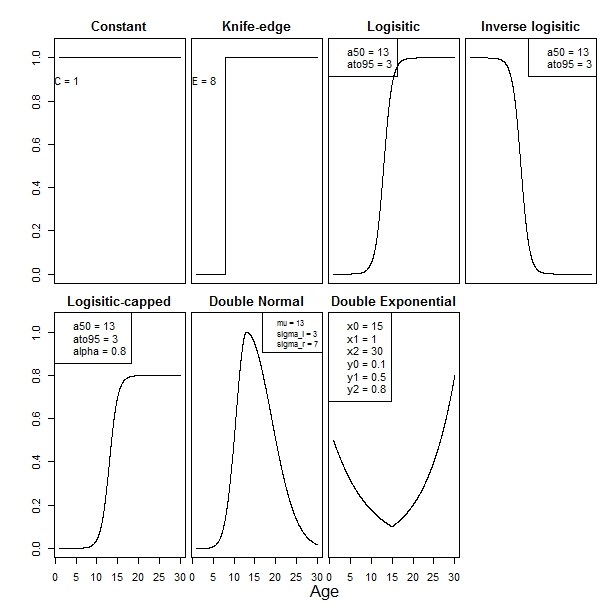
\includegraphics[scale = 0.7]{Figures/Selectivities.jpeg}
	\caption{Examples of the functional forms of selectivities available in \CNAME.}
\end{figure}

\subsection{\I{Time Varying Parameters}\label{sec:time_var}}

\CNAME\ has the functionality to vary a parameter annually between the start and final year of a model run. This can be for blocks of years or specific years if chosen. For years that are not specified the parameter will default to the input or if in a iterative state such as estimation mode, the value being trialled at that iteration. Available methods for time varying a parameter. Where this functionality will become quite useful is in simulating more realistic observations. When you allow fisheries to have annual varying catchabilities and other more realistic model components simulated observations become more real data and thus conclusions based on simulated data are more useful.

\subsubsection[Constant]{\argument{Constant}}\index{Time Varying Parameters!Constant}
Allows a parameter to have an alternative values during certain years, which can be estimated.
{\small{\begin{verbatim}
		@time_varying q_time_var
		type constant
		parameter catchability[survey_q].q
		years 1975:1988
		value 0.001
		\end{verbatim}}}

\subsubsection[Random Walk]{\argument{Random Walk}}\index{Time Varying Parameters!Random Walk}

A random deviate added into the last value drawn from a standard normal distribution. This has an estimable parameter $\sigma_p$ for each time varying parameter $p$. For reproducible modelling, it is highly recommended that users set the seed (see Section~\ref{sec:command-line-arguments}) when using stochastic functionality like this, otherwise reproducing models becomes almost impossible.
{\small{\begin{verbatim}
		@time_varying q_time_var
		type random_walk
		parameter catchability[survey_q].q
		distribution normal
		mean 0
		sigma 3
		\end{verbatim}}}

If the \texttt{parameter} specified in the \command{time\_varying} is associated with an \command{estimate} block then the parameter is constrained to stay within the lower and upper bounds of the \command{estimate} block. Warning, if the parameter does not have an associated \command{estimate} block then there is no safe guard for a random deviate to put the parameter in a space where the model fails, i.e generates NA or INF values. to avoid this from happening it is recommended you specify an \command{estimate} block even though you are not estimating the parameter like below.

{\small{\begin{verbatim}
		@estimate survey_q_est
		type uniform
		parameter catchability[survey_q].q
		lower_bound 1e-6
		upper_bound 10
		\end{verbatim}}}
This will insure the random walk time varying process will set the any new candidate within the lower and upper bound of the \command{estimate} block.

\subsubsection[Annual shift]{\argument{Annual shift}}\index{Time Varying Parameters!Annual shift}
A parameter generated in year $y$ ($\theta'_y$) depends on the value specified by the user ($\theta_y$) along with three coefficients $a,b$ and $c$ as follows,

\begin{equation}
\bar{\theta}_y = \frac{\sum_{y}^Y\theta_y}{Y}
\end{equation}

\begin{equation}
\theta'_y = a \bar{\theta}_y + b\bar{\theta}_y^{2} + c\bar{\theta}_y^{3}
\end{equation}

\subsubsection[Exogenous]{\argument{Exogenous}}\index{Time Varying Parameters!Exogenous}

Parameters are shifted based on an exogenous variable, an example of this is an exploitation selectivity parameters that may vary between years based on known changes in exploitation behaviour such as season, start time, and average depth of exploitation.
\begin{equation}
\delta_y = a(E_y - \bar{E})
\end{equation}

\begin{equation}
\theta'_y = \theta_y + \delta_y
\end{equation}
where $\delta_y$ is the shift or deviation in parameter $\theta_y$ in year $y$ to generate the new parameter value in year $y$ ($\theta'_y$). $a$ is an estimable shift parameter, $E$ is the exogenous variable and $E_y$ is the value of this variable in year $y$. For more information readers can see \cite{francis_03}.

